\chapter{Lagrangian Subhalo Cores, Self-Unbinding, and a Tidal-Survival Audit}
\label{ch:subhalo-core-tidal-audit}
\newcommand{\SCTPass}{20}
\newcommand{\SCTFail}{0}
\newcommand{\SCTCandidates}{27}
\newcommand{\SCTRobust}{23}
\newcommand{\SCTBoundRatio}{0.958333}
\newcommand{\SCTBoundMassZoom}{0.943218}
\newcommand{\SCTBoundMassFine}{0.946203}
\newcommand{\SCTRhalfZoom}{0.975744}
\newcommand{\SCTRhalfFine}{0.963235}
\newcommand{\SCTVmaxZoom}{1.004713}
\newcommand{\SCTVmaxFine}{1.005865}
\newcommand{\SCTHardZoom}{0.772727}
\newcommand{\SCTHardFine}{0.900000}
\newcommand{\SCTSmoothZoomMin}{1.098323}
\newcommand{\SCTSmoothZoomMed}{1.126285}
\newcommand{\SCTSmoothZoomMax}{1.178158}
\newcommand{\SCTSmoothFineMin}{1.101874}
\newcommand{\SCTSmoothFineMed}{1.128740}
\newcommand{\SCTSmoothFineMax}{1.178707}
\newcommand{\SCTLumZoomMin}{1.078604}
\newcommand{\SCTLumZoomMed}{1.120992}
\newcommand{\SCTLumZoomMax}{1.193886}
\newcommand{\SCTLumFineMin}{1.091975}
\newcommand{\SCTLumFineMed}{1.125179}
\newcommand{\SCTLumFineMax}{1.188766}
\newcommand{\SCTStellarZoomMin}{1.018648}
\newcommand{\SCTStellarZoomMed}{1.034769}
\newcommand{\SCTStellarZoomMax}{1.051922}
\newcommand{\SCTStellarFineMin}{1.006992}
\newcommand{\SCTStellarFineMed}{1.025213}
\newcommand{\SCTStellarFineMax}{1.040640}
\newcommand{\SCTCompactZoom}{0.994943}
\newcommand{\SCTCompactFine}{0.981155}


\section{Scope and objective}

The preceding nonlinear calculation resolved paired halo catalogues and showed that near-cutoff refinement halos are less massive, have lower maximum circular-speed proxies, and assemble later than their cold counterparts.  The one-zone baryonic section then showed that these gravitational differences can strongly suppress dwarf stellar activity and high-redshift ionizing production.  A true satellite prediction, however, requires a different object: a self-bound remnant inside a larger host rather than an isolated friends-of-friends component.

This chapter constructs a controlled Lagrangian subhalo-core audit.  It uses particle identities to select matched accreted progenitors at $a=0.5$, follows their particles into five paired host halos at $a=1$, applies a finite spherical self-unbinding map, and compares the resulting cold and refinement remnants.  It then subjects those remnants to a declared tide, disk, and baryonic response envelope.

The principal result is mixed and therefore important:
\begin{equation}
\boxed{
\begin{gathered}
\text{matched refinement remnants contain less bound mass and are slightly smaller},\\
\text{their }V_{\max}\text{ and velocity dispersion remain nearly cold-like},\\
\text{resolved self-bound core counts are almost unchanged},\\
\text{and the sign of a satellite-count correction depends on the unresolved stripping model}.
\end{gathered}}
\label{eq:sct-central-result}
\end{equation}

Thus the present calculation does not support a universal statement that the refinement branch must contain fewer surviving satellites.  It identifies a robust remnant-structure signal and a precise numerical boundary on satellite-count claims.

\section{Matched accreted progenitors}

Let $H_C$ and $H_R$ be a matched cold/refinement host pair at $a=1$.  Let $E_C$ and $E_R$ be a matched pair of halos at $a=0.5$.  The retained accreted-progenitor sample requires:
\begin{align}
N(E_C),N(E_R)&\ge 64,\label{eq:sct-ninit}\\
J(E_C,E_R)&\ge0.2,\label{eq:sct-jaccard}\\
f_{\rm desc,C},f_{\rm desc,R}&\ge0.5,\label{eq:sct-desc}\\
D(E_C)&=H_C,\qquad D(E_R)=H_R.\label{eq:sct-desc-host}
\end{align}
Here $J$ is the particle-ID Jaccard overlap and $D$ is the largest-particle-overlap descendant map.  The principal progenitor of each host is removed so that the sample represents accreted systems rather than the host itself.

The construction gives
\begin{equation}
\boxed{\SCTCandidates\ \text{matched accreted progenitor pairs}}
\label{eq:sct-candidate-count}
\end{equation}
in both the $260$-step run and its $360$-step time control.  After requiring at least twenty self-bound particles in both members of a pair, the structural sample contains
\begin{equation}
\boxed{\SCTRobust\ \text{robust matched remnant pairs}.}
\label{eq:sct-robust-count}
\end{equation}

This Lagrangian construction is stronger than counting neighboring field halos.  Every retained remnant is tied to a declared progenitor and a declared final host by particle identities.

\section{Finite spherical self-unbinding}

For a candidate particle set $S$, choose a robust center $x_S$ and inner-core velocity $v_S$.  For particle $i\in S$, set
\begin{equation}
r_i=\lVert x_i-x_S\rVert,
\qquad
K_i(S)=\frac12\lVert v_i-v_S\rVert^2.
\label{eq:sct-kinetic}
\end{equation}
In the spherical shell approximation, the potential is
\begin{equation}
\Phi_i(S)
=-G\left[
\frac{M_S(\le r_i)}{r_i}
+
\sum_{j\in S:\,r_j>r_i}\frac{m_p}{r_j}
\right].
\label{eq:sct-potential}
\end{equation}
The declared energy criterion is
\begin{equation}
E_i(S)=K_i(S)+\Phi_i(S).
\label{eq:sct-energy}
\end{equation}
Starting from the particles of the early halo that enter the selected final host, define
\begin{equation}
S_{n+1}
=
\{i\in S_n:E_i(S_n)<0\}.
\label{eq:sct-unbinding-map}
\end{equation}

\subsection{Finite-termination theorem}

\textbf{Theorem 61.1.}
For a finite initial set $S_0$, the self-unbinding sequence in \eqref{eq:sct-unbinding-map} stabilizes after at most $|S_0|$ strict-removal steps.

\textbf{Proof.}
By construction,
\begin{equation}
S_{n+1}\subseteq S_n.
\label{eq:sct-nested}
\end{equation}
If the inclusion is strict, at least one particle is removed.  A finite set admits at most $|S_0|$ such removals.  Hence there is an $N\le|S_0|$ with $S_{N+1}=S_N$.  At this fixed point, every retained particle satisfies the declared negative-energy criterion.  \hfill$\square$

The theorem proves finite algorithmic closure.  It does not prove that the fixed point is independent of the center prescription, spherical approximation, force softening, or temporal sampling.

For a stabilized set $S_\infty$, define
\begin{align}
M_b&=m_p|S_\infty|,\label{eq:sct-bound-mass}\\
r_{1/2}&=\operatorname{median}_{i\in S_\infty}r_i,\label{eq:sct-rhalf}\\
\sigma_{1\rm D}^2&=\frac1{3|S_\infty|}\sum_{i\in S_\infty}\lVert v_i-v_S\rVert^2,\label{eq:sct-sigma}\\
V_{\max}^{\rm proxy}&=\sqrt{\frac{GM_b}{r_{1/2}}}.\label{eq:sct-vmax}
\end{align}
The last quantity is a compact structural proxy rather than a converged circular-speed curve.

\section{Resolved self-bound core counts}

The particle-threshold counts are shown in Figure~\ref{fig:sct-thresholds}.  At the central threshold $N_b\ge20$, both time resolutions give
\begin{equation}
\boxed{
N_{C}=24,
\qquad
N_{R}=23,
\qquad
\frac{N_R}{N_C}=\SCTBoundRatio.
}
\label{eq:sct-bound-count}
\end{equation}
At $N_b\ge64$, both branches contain twenty-two remnants in both runs.  Thus the resolved core-count deficit is only one object at the central threshold and disappears at the higher threshold.

\begin{figure}[htbp]
\centering
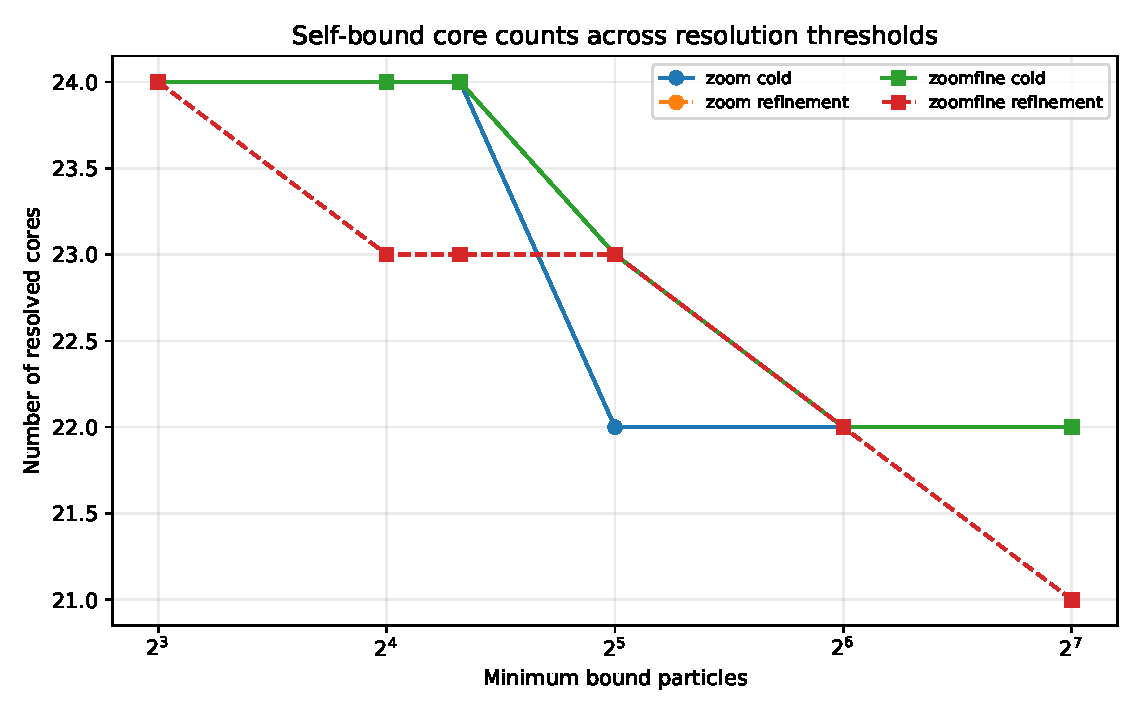
\includegraphics[width=.84\linewidth]{figures/sub/01_bound_core_thresholds.pdf}
\caption{Self-bound remnant counts as the minimum particle threshold is raised.  The cold and refinement curves remain close in both the principal and time-control calculations.}
\label{fig:sct-thresholds}
\end{figure}

This is already a correction to the earlier field-halo intuition.  A deficit in isolated near-cutoff halos does not map one-to-one into a deficit of resolved bound cores inside hosts.

\section{Matched core structure}

For the twenty-three pairs resolved above twenty particles in both branches, the median structural ratios are
\begin{center}
\begin{tabular}{lcc}
\toprule
observable & $260$-step run & $360$-step control\\
\midrule
$M_{b,R}/M_{b,C}$ & \SCTBoundMassZoom & \SCTBoundMassFine\\
$r_{1/2,R}/r_{1/2,C}$ & \SCTRhalfZoom & \SCTRhalfFine\\
$V_{\max,R}/V_{\max,C}$ & \SCTVmaxZoom & \SCTVmaxFine\\
$\sigma_{1\rm D,R}/\sigma_{1\rm D,C}$ & 1.023202 & 1.013546\\
\bottomrule
\end{tabular}
\end{center}

The mass ratios differ between the two time resolutions by less than $0.003$, and the half-mass-radius ratios differ by about $0.013$.  The result is therefore stable at the scale of the present pilot:
\begin{equation}
\boxed{
M_{b,R}\simeq0.945M_{b,C},
\qquad
r_{1/2,R}\simeq0.97r_{1/2,C},
\qquad
V_{\max,R}\simeq V_{\max,C}.
}
\label{eq:sct-structure-summary}
\end{equation}

\begin{figure}[htbp]
\centering
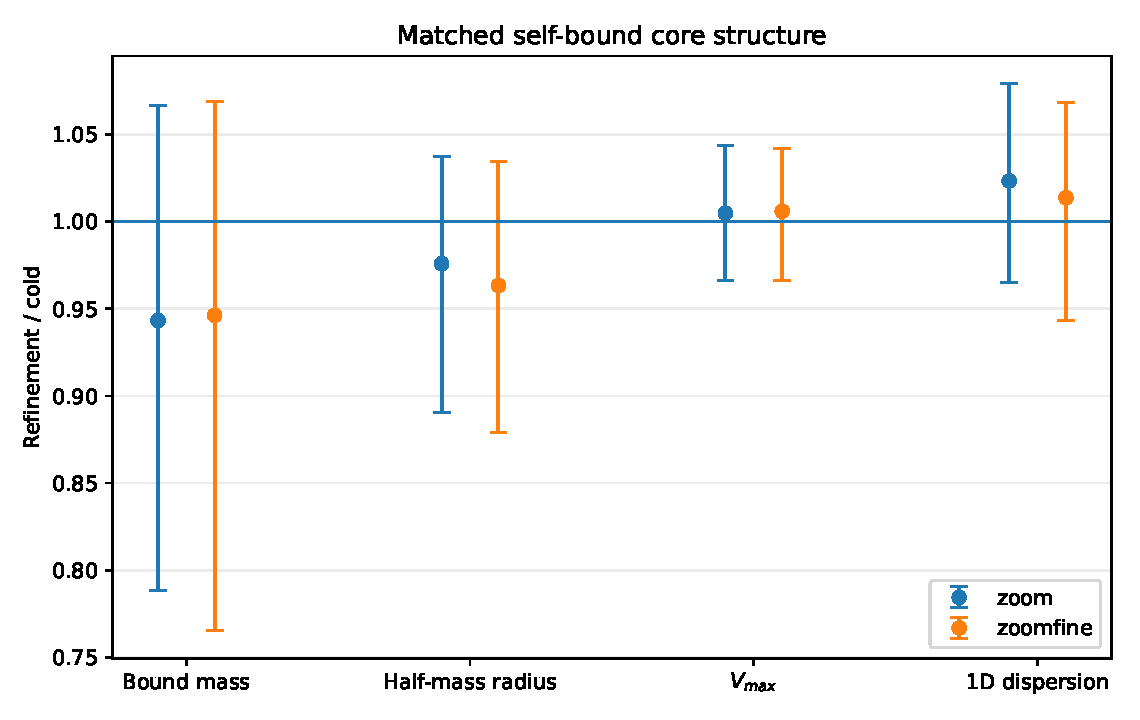
\includegraphics[width=.84\linewidth]{figures/sub/02_core_structure_ratios.pdf}
\caption{Median refinement-to-cold core ratios with $16$th--$84$th percentile intervals.  Bound mass and radius are mildly reduced, while the velocity proxies remain close to unity.}
\label{fig:sct-structure-ratios}
\end{figure}

Approximately seventy percent of the matched remnants have $r_{1/2,R}<r_{1/2,C}$.  The object-by-object mass-size relation is shown in Figure~\ref{fig:sct-mass-size}.

\begin{figure}[htbp]
\centering
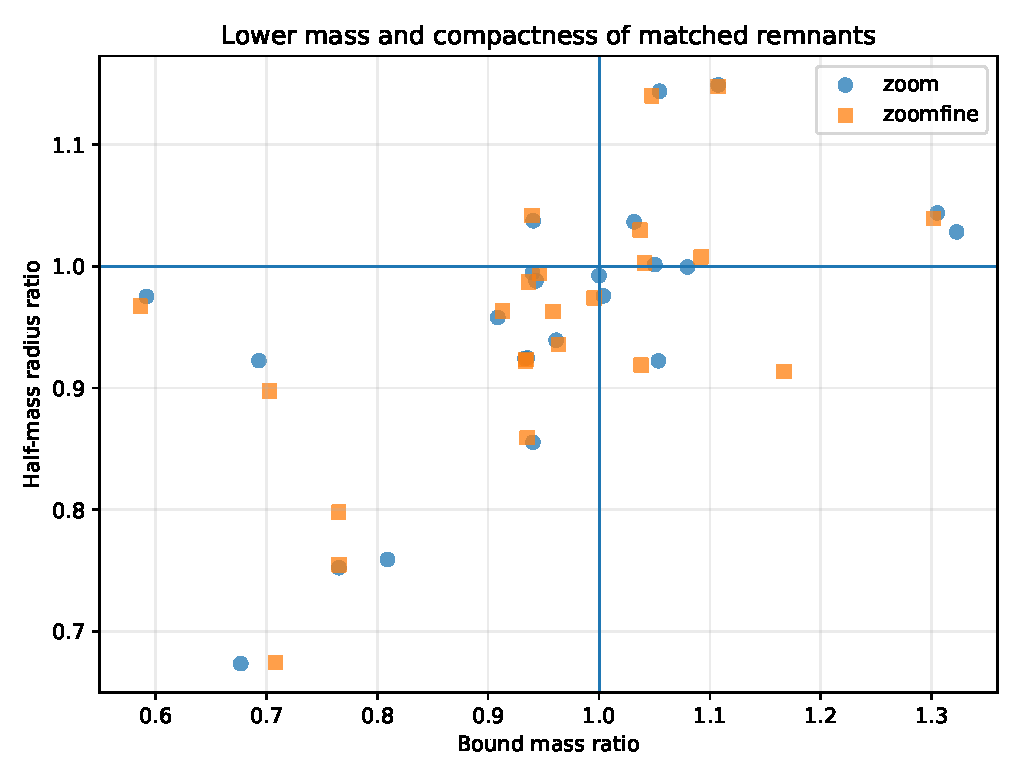
\includegraphics[width=.74\linewidth]{figures/sub/03_mass_size_scatter.pdf}
\caption{Matched bound-mass and half-mass-radius ratios.  The dominant tendency is toward a lower-mass, slightly smaller refinement remnant, although substantial object-to-object scatter remains.}
\label{fig:sct-mass-size}
\end{figure}

\section{Compactness compensation}

For equal host orbit and tidal coefficient, the Jacobi-like tidal radius scales as
\begin{equation}
r_t
=R\left(\frac{M_b}{\kappa M_{\rm host}(<R)}\right)^{1/3}.
\label{eq:sct-rt-simple}
\end{equation}
The ratio of the size-to-tidal-radius variables is therefore
\begin{equation}
\frac{(r_{1/2}/r_t)_R}{(r_{1/2}/r_t)_C}
=
\frac{r_{1/2,R}/r_{1/2,C}}
{(M_{b,R}/M_{b,C})^{1/3}}.
\label{eq:sct-compactness-factor}
\end{equation}
At the median this factor is
\begin{equation}
\boxed{
\mathcal K_{260}=\SCTCompactZoom,
\qquad
\mathcal K_{360}=\SCTCompactFine.
}
\label{eq:sct-compactness-values}
\end{equation}
Both are below unity.  The reduction in physical size compensates for the reduction in mass, so the typical refinement core is not automatically more vulnerable to a common tidal field.

This mechanism explains why a field-halo deficit need not survive as a satellite-core deficit.  The systems that do form in the refinement branch are selected from a colder and more compact surviving population.

\section{Hard current-position tidal proxy}

A separate hard truncation was also applied at the current host-centric radius.  At the twenty-particle threshold it gives
\begin{equation}
\boxed{
\left.\frac{N_R}{N_C}\right|_{\rm hard,260}=\SCTHardZoom,
\qquad
\left.\frac{N_R}{N_C}\right|_{\rm hard,360}=\SCTHardFine.
}
\label{eq:sct-hard-count}
\end{equation}
This proxy suggests fewer refinement remnants, but it changes from $0.773$ to $0.900$ under the time control.  Its sign is stable, but its magnitude is not converged sufficiently for a satellite likelihood.

The hard proxy is sensitive to particle discretization near a sharp tidal boundary.  It should be treated as a negative-control estimate rather than a final count.

\section{Smooth tide, disk, and shock envelope}

To test whether the conclusion depends on sharp truncation, introduce an exponential host disk with mass fraction $f_d$ and scale radius $R_d$.  Its spherical-equivalent enclosed mass is
\begin{equation}
M_d(<R)
=f_dM_{\rm host}\left[1-\left(1+\frac{R}{R_d}\right)e^{-R/R_d}\right].
\label{eq:sct-disk-mass}
\end{equation}
The declared tidal radius is
\begin{equation}
r_t
=R\left[
\frac{M_b}{\kappa\{M_{\rm host}(<R)+M_d(<R)\}}
\right]^{1/3}.
\label{eq:sct-tidal-radius}
\end{equation}
Define the smooth tidal survival weight
\begin{equation}
w_t
=\left[1+\left(\frac{2r_{1/2}}{r_t}\right)^4\right]^{-1}.
\label{eq:sct-tidal-weight}
\end{equation}
A disk-shock proxy is
\begin{equation}
\Xi
=\left[
\frac{2GM_d(<R)r_{1/2}}
{R^2v_{\rm rel}V_{\max}}
\right]^2,
\qquad
w_s=e^{-A\Xi},
\label{eq:sct-shock}
\end{equation}
so that
\begin{equation}
w_{\rm surv}=w_tw_s.
\label{eq:sct-survival-weight}
\end{equation}

The scan contains $144$ tide/disk choices per time resolution:
\begin{equation}
\begin{gathered}
f_d\in\{0,0.01,0.03,0.05\},
\qquad
R_d/r_{90}\in\{0.03,0.06,0.10\},\\
\kappa\in\{2,3,5\},
\qquad
A\in\{0,0.5,1,2\}.
\end{gathered}
\label{eq:sct-gravity-grid}
\end{equation}

The resulting refinement-to-cold survival envelopes are
\begin{equation}
\boxed{
\SCTSmoothZoomMin
\leq
\frac{\sum_iw_{i,R}}{\sum_iw_{i,C}}
\leq
\SCTSmoothZoomMax,
\qquad
\operatorname{median}=\SCTSmoothZoomMed
}
\label{eq:sct-smooth-zoom}
\end{equation}
for the principal run and
\begin{equation}
\boxed{
\SCTSmoothFineMin
\leq
\frac{\sum_iw_{i,R}}{\sum_iw_{i,C}}
\leq
\SCTSmoothFineMax,
\qquad
\operatorname{median}=\SCTSmoothFineMed
}
\label{eq:sct-smooth-fine}
\end{equation}
for the time control.

Every model in this declared smooth envelope lies above unity.  The smaller refinement-core sizes outweigh their lower masses in the survival weighting.  Figure~\ref{fig:sct-disk-scan} shows that this compensation persists as the disk fraction is increased.

\begin{figure}[htbp]
\centering
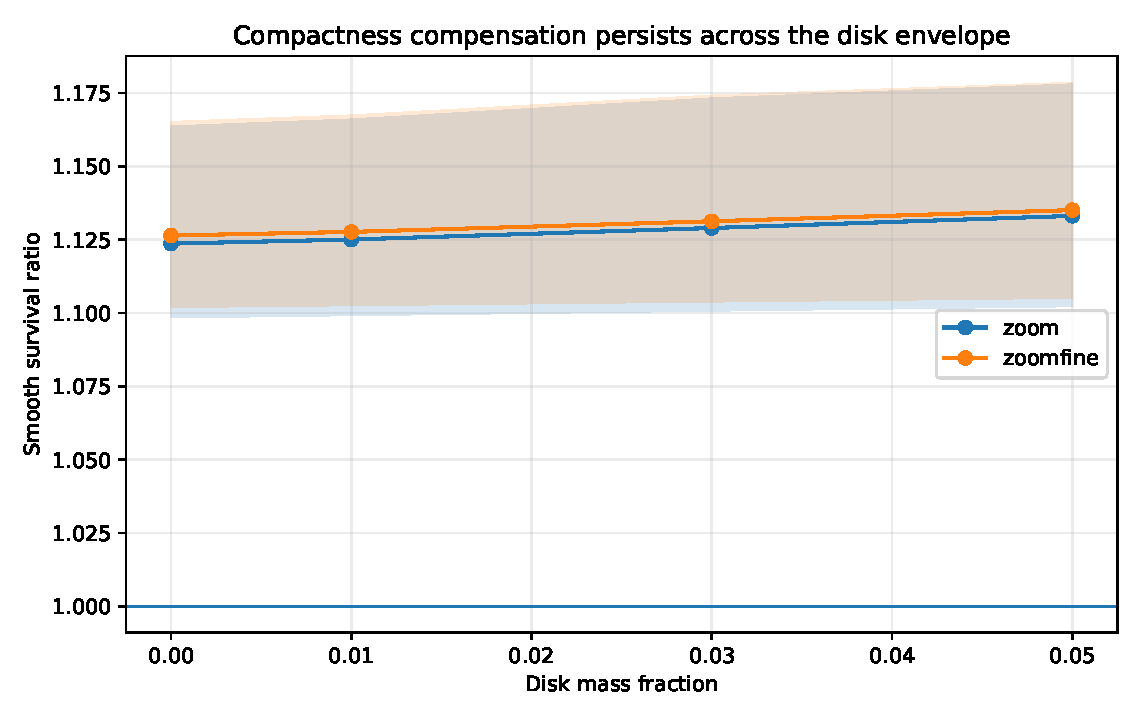
\includegraphics[width=.82\linewidth]{figures/sub/06_disk_fraction_scan.pdf}
\caption{Median and full range of the smooth survival ratio versus disk mass fraction.  Compactness compensation persists throughout the declared tide and shock envelope.}
\label{fig:sct-disk-scan}
\end{figure}

\section{Luminous and stellar survival weights}

A common luminous occupation map is
\begin{equation}
P_{\rm lum}(V)
=\left[
1+\exp\left(-\frac{\log(V/V_{50})}{s}\right)
\right]^{-1}.
\label{eq:sct-luminous-map}
\end{equation}
Scanning
\begin{equation}
V_{50}\in\{15,20,25,30,40\}\ {\rm km\,s^{-1}},
\qquad
s\in\{0.15,0.25,0.40,0.60\},
\label{eq:sct-occ-grid}
\end{equation}
gives the surviving luminous-weight envelopes
\begin{align}
\SCTLumZoomMin
&\leq R_{\rm lum}^{260}\leq\SCTLumZoomMax,
&\operatorname{median}R_{\rm lum}^{260}&=\SCTLumZoomMed,\label{eq:sct-lum-zoom}\\
\SCTLumFineMin
&\leq R_{\rm lum}^{360}\leq\SCTLumFineMax,
&\operatorname{median}R_{\rm lum}^{360}&=\SCTLumFineMed.\label{eq:sct-lum-fine}
\end{align}

A common feedback-weighted stellar proxy uses
\begin{equation}
\epsilon_\star(V)
=C_{\rm atom}(V)C_{\rm ph}(V)
\frac{1-\mathcal R}{1-\mathcal R+(V_{\rm fb}/V)^\beta}.
\label{eq:sct-stellar-efficiency}
\end{equation}
Across thirty-six feedback choices per gravity model, the integrated surviving stellar-weight envelopes are
\begin{align}
\SCTStellarZoomMin
&\leq R_\star^{260}\leq\SCTStellarZoomMax,
&\operatorname{median}R_\star^{260}&=\SCTStellarZoomMed,\label{eq:sct-star-zoom}\\
\SCTStellarFineMin
&\leq R_\star^{360}\leq\SCTStellarFineMax,
&\operatorname{median}R_\star^{360}&=\SCTStellarFineMed.\label{eq:sct-star-fine}
\end{align}

These ratios also exceed unity in the smooth envelope.  They should not be interpreted as a prediction of more observed satellites.  They show that common compactness-dependent survival can offset, and in this model family reverse, the earlier field-halo and dwarf-formation suppression.

\begin{figure}[htbp]
\centering
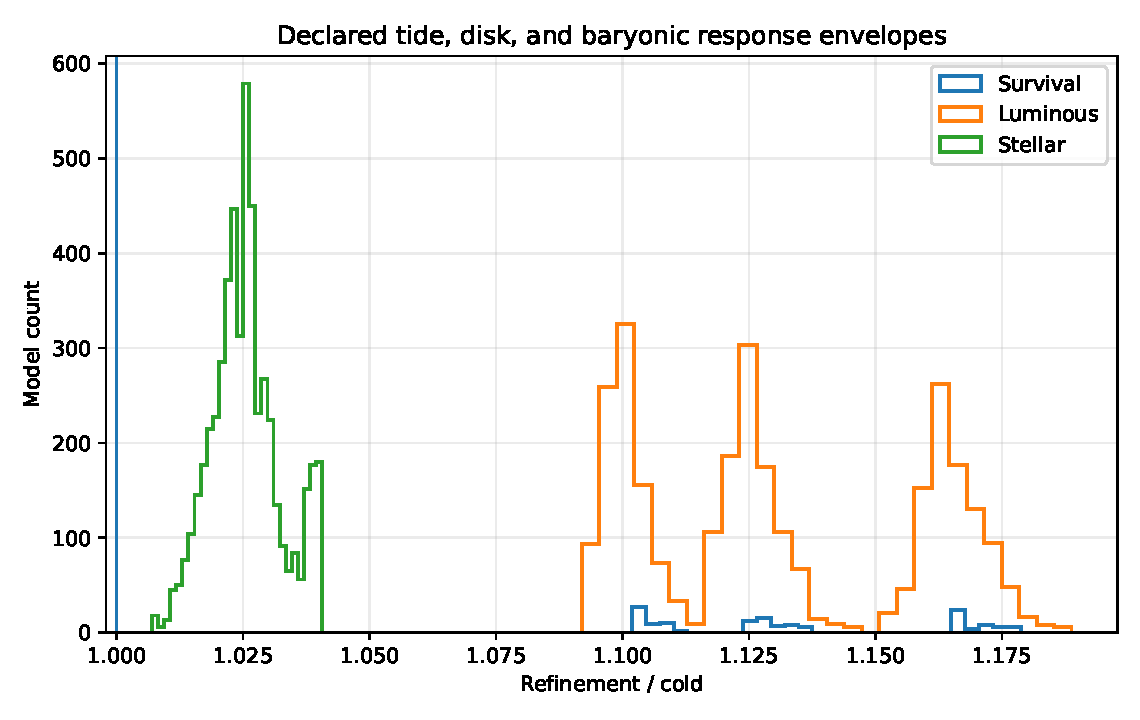
\includegraphics[width=.84\linewidth]{figures/sub/05_survival_envelopes.pdf}
\caption{Distribution of the smooth survival, luminous, and stellar ratios in the $360$-step control.  Every declared model lies above unity, in direct tension with the hard truncation proxy.}
\label{fig:sct-envelope-hist}
\end{figure}

\section{Proxy disagreement and the satellite boundary}

The three retained remnant diagnostics give
\begin{center}
\begin{tabular}{lcc}
\toprule
proxy & $260$-step run & $360$-step control\\
\midrule
self-bound core count, $N_b\ge20$ & 0.958333 & 0.958333\\
hard current tidal count, $N\ge20$ & \SCTHardZoom & \SCTHardFine\\
smooth tide/disk survival envelope & $\SCTSmoothZoomMin$--$\SCTSmoothZoomMax$ & $\SCTSmoothFineMin$--$\SCTSmoothFineMax$\\
\bottomrule
\end{tabular}
\end{center}

The proxies straddle unity.  This is not a nuisance to be hidden.  It is the decisive result of the section:
\begin{equation}
\boxed{
\begin{gathered}
\text{the present spatial and temporal resolution does not determine}\\
\text{the sign of the satellite-count correction}
\end{gathered}
}
\label{eq:sct-no-sign}
\end{equation}

\begin{figure}[htbp]
\centering
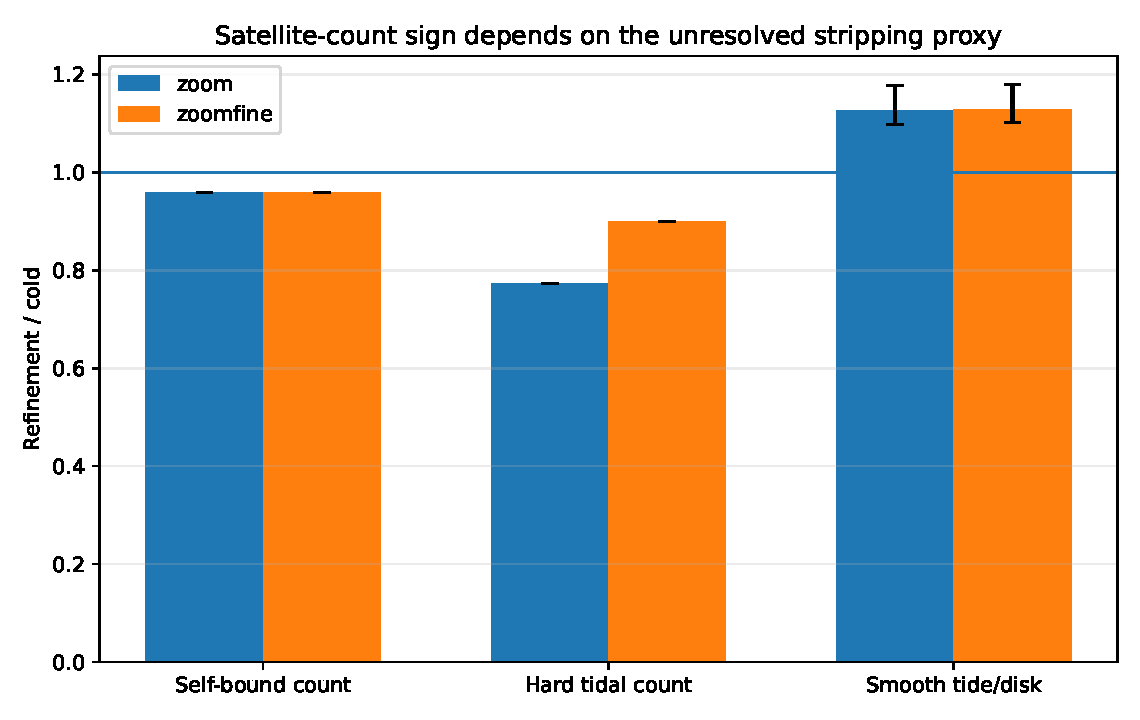
\includegraphics[width=.84\linewidth]{figures/sub/04_proxy_disagreement.pdf}
\caption{The self-bound count, hard tidal cut, and smooth tide/disk envelope do not give one common satellite-count sign.  A resolved host zoom and subhalo finder are required before a satellite likelihood is defensible.}
\label{fig:sct-proxy-disagreement}
\end{figure}

What remains robust is the structural statement:
\begin{equation}
\boxed{
\begin{gathered}
\text{matched refinement remnants are mildly less massive and smaller,}\\
\text{but retain nearly cold-like central velocity scales}
\end{gathered}
}
\label{eq:sct-robust-claim}
\end{equation}

\section{Verification ledger}

The deterministic audit records
\begin{equation}
\boxed{
\SCTPass\ {\rm PASS},
\qquad
\SCTFail\ {\rm FAIL}.
}
\label{eq:sct-pass-count}
\end{equation}
It checks the paired-sample definition, overlap and descendant thresholds, finite self-unbinding termination, particle-threshold counts, structural time control, compactness compensation, finite response scans, and the proxy sign disagreement.

The complete scan contains
\begin{equation}
288\ \text{gravity rows},
\qquad
5760\ \text{luminous rows},
\qquad
10368\ \text{stellar rows}.
\label{eq:sct-scan-counts}
\end{equation}
All archived ratios are finite.

\section{Claim boundary}

This chapter establishes:
\begin{itemize}
\item an exact finite-termination theorem for the declared self-unbinding map;
\item particle-ID-selected accreted progenitor pairs in two time resolutions;
\item controlled self-bound count and matched-structure ratios;
\item a compactness-compensation diagnostic;
\item a declared smooth tide, disk, luminous, and stellar response envelope;
\item a negative result showing that the satellite-count sign is unresolved.
\end{itemize}

It does not establish:
\begin{itemize}
\item a force- and particle-converged subhalo mass function;
\item a six-dimensional phase-space subhalo finder;
\item resolved pericentric stripping or repeated tidal shocks;
\item a live baryonic disk, hydrodynamics, or disk shocking;
\item complete merger trees, orphan satellites, or disruption histories;
\item a survey selection function or satellite likelihood;
\item a microscopic derivation of the refinement production parameters.
\end{itemize}
